\chapter[Experimentos e Análise dos Resultados]{Experimentos e Análise dos Resultados}
\label{experimentos}

Este capítulo apresenta a avaliação experimental dos métodos descritos no Capítulo~\ref{proposta}. A análise usa os arquivos estruturados produzidos pela implementação: \TotalArquivosResumo{} resumos, \TotalArquivosEvolucao{} históricos de evolução e \TotalArquivosTempo{} arquivos de tempo. Os resultados são discutidos em termos de qualidade da solução, tempo computacional, estabilidade entre sementes, significância estatística e limitações metodológicas.

\section{Método para a Avaliação}
\label{metodo}

Todas as execuções otimizam a mesma função objetivo: o \textit{makespan} da rota de patrulhamento. Uma solução factível parte da base, visita cada ponto de interesse exatamente uma vez e retorna à base. A avaliação usa o tensor $G[anterior][atual][proximo]$, que incorpora distância euclidiana e penalidade angular.

As instâncias são sintéticas, com coordenadas no intervalo $[-1,1]$. Foram usados \TotalTamanhosInstancia{} tamanhos de instância, com \TotalVariantesPorTamanho{} variantes por tamanho, totalizando \TotalInstancias{} instâncias. GA, PSO e ACO foram executados com \TotalSementesGA{} sementes em cada instância. A busca exaustiva foi executada nas \TotalInstanciasComOtimo{} instâncias de 10 a 15 pontos. O lower bound AP foi executado em todas as \TotalInstancias{} instâncias.

As métricas principais são:
\begin{itemize}
  \item \textbf{makespan}: valor final da função objetivo;
  \item \textbf{gap vs. ótimo}: diferença percentual em relação à busca exaustiva, nas 18 instâncias com ótimo conhecido;
  \item \textbf{gap vs. lower bound}: diferença percentual em relação ao limitante AP;
  \item \textbf{tempo de otimização}: duração da etapa de otimização em milissegundos;
  \item \textbf{taxa de acerto}: proporção de sementes que alcançam o ótimo nas instâncias com busca exaustiva.
\end{itemize}

\begin{table}[htbp]
  \centering
  \caption{Cobertura experimental dos métodos avaliados.}
  \label{tab:cobertura-experimental}
  % Generated by scripts/gerar-metricas-monografia.py; do not edit manually.
% Source: src/data/results via scripts/gerar-metricas-monografia.py.
\begin{tabular}{lrrr}
\toprule
Metodo & Runs & Instancias & Sementes \\
\midrule
ACO & 1530 & 30 & 51 \\
GA & 1530 & 30 & 51 \\
PSO & 1530 & 30 & 51 \\
Lower bound & 30 & 30 & 1 \\
Busca exaustiva & 18 & 18 & 1 \\
\bottomrule
\end{tabular}

\end{table}

\section{Experimentos}

Os experimentos foram executados por uma interface de linha de comando em Go. Cada execução recebe o arquivo de instância, o método, a semente e o diretório de resultados. O identificador da execução é usado para nomear os arquivos de resumo, evolução e tempo. Para as meta-heurísticas, os parâmetros foram mantidos fixos: população 100 e 100 iterações. Essa decisão permite comparar os métodos sob o mesmo orçamento populacional, mas não substitui uma análise de sensibilidade de hiperparâmetros.

A busca exaustiva fornece o ótimo global nas instâncias em que foi executada. A Tabela~\ref{tab:otimos-bf} apresenta esses valores. Eles são usados como referência para calcular o gap das meta-heurísticas nas instâncias pequenas.

\begin{table}[htbp]
  \centering
  \caption{Ótimos obtidos por busca exaustiva nas 18 instâncias pequenas.}
  \label{tab:otimos-bf}
  \scriptsize
  % Generated by scripts/gerar-metricas-monografia.py; do not edit manually.
% Source: src/data/results via scripts/gerar-metricas-monografia.py.
\begin{tabular}{rrrrrr}
\toprule
Instancia & Otimo & Instancia & Otimo & Instancia & Otimo \\
\midrule
10a & 8{,}251 & 10b & 7{,}906 & 10c & 9{,}545 \\
11a & 9{,}493 & 11b & 8{,}823 & 11c & 10{,}260 \\
12a & 9{,}501 & 12b & 9{,}769 & 12c & 10{,}480 \\
13a & 10{,}950 & 13b & 11{,}474 & 13c & 10{,}042 \\
14a & 11{,}557 & 14b & 11{,}467 & 14c & 11{,}486 \\
15a & 9{,}129 & 15b & 12{,}185 & 15c & 12{,}160 \\
\bottomrule
\end{tabular}

\end{table}

\section{Avaliação dos Resultados}
\label{avaliacao}

\subsection{Qualidade nas Instâncias com Ótimo Conhecido}

Nas \TotalInstanciasComOtimo{} instâncias com busca exaustiva, o ACO apresentou o menor gap médio em relação ao ótimo. A Tabela~\ref{tab:gap-bf} resume os resultados agregados sobre \TotalExecucoesOtimoPorMetodo{} execuções por método nesse subconjunto. O ACO obteve gap médio de \GapMedioOtimoACO{} e taxa global de acerto de \TaxaAcertoOtimoACO{}. O GA obteve gap médio de \GapMedioOtimoGA{} e taxa de acerto de \TaxaAcertoOtimoGA{}. O PSO obteve gap médio de \GapMedioOtimoPSO{} e taxa de acerto de \TaxaAcertoOtimoPSO{}.

\begin{table}[htbp]
  \centering
  \caption{Gap percentual em relação ao ótimo nas instâncias `10a'--`15c'.}
  \label{tab:gap-bf}
  % Generated by scripts/gerar-metricas-monografia.py; do not edit manually.
% Source: src/data/results via scripts/gerar-metricas-monografia.py.
\begin{tabular}{lrrrrr}
\toprule
Metodo & Runs & Gap medio & Gap min. & Gap max. & Taxa de acerto \\
\midrule
ACO & 918 & 0{,}4296\% & 0{,}0000\% & 9{,}4445\% & 71{,}79\% \\
GA & 918 & 5{,}2814\% & 0{,}0000\% & 41{,}4267\% & 26{,}47\% \\
PSO & 918 & 22{,}2915\% & 0{,}0000\% & 76{,}5549\% & 4{,}25\% \\
\bottomrule
\end{tabular}

\end{table}

\begin{figure}[htbp]
  \centering
  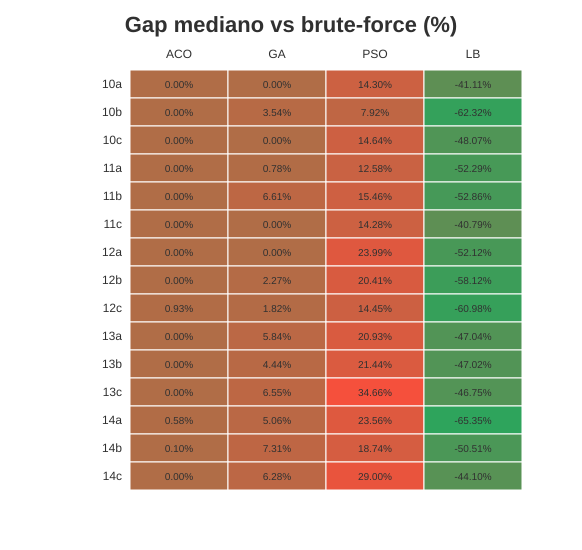
\includegraphics[width=0.86\textwidth]{figs/heatmap-gap-vs-bf.png}
  \caption{Gap em relação à busca exaustiva nas instâncias com ótimo conhecido. Fonte: dados de `src/data/results/'.}
  \label{fig:gap-vs-bf}
\end{figure}

\begin{figure}[htbp]
  \centering
  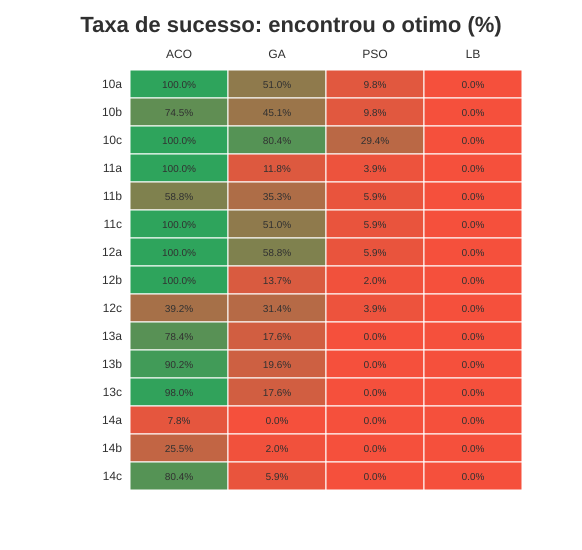
\includegraphics[width=0.86\textwidth]{figs/heatmap-success-rate.png}
  \caption{Taxa de acerto do ótimo por método nas instâncias pequenas. Fonte: dados de `src/data/results/'.}
  \label{fig:taxa-acerto}
\end{figure}

\subsection{Qualidade nas Instâncias Maiores}

Para instâncias acima de 15 pontos, a busca exaustiva não foi usada como ótimo de referência. A análise passa a comparar as meta-heurísticas entre si e com o lower bound. Nas instâncias de 50 e 100 pontos, o ACO apresentou \textit{makespan} médio substancialmente menor que GA e PSO, como mostra a Tabela~\ref{tab:grandes}.

\begin{table}[htbp]
  \centering
  \caption{Melhor e média de makespan nas instâncias de 50 e 100 pontos.}
  \label{tab:grandes}
  \scriptsize
  % Generated by scripts/gerar-metricas-monografia.py; do not edit manually.
% Source: src/data/results via scripts/gerar-metricas-monografia.py.
\begin{tabular}{lrrrrrr}
\toprule
Instancia & ACO best & ACO media & GA best & GA media & PSO best & PSO media \\
\midrule
50a & 24{,}6688 & 25{,}6475 & 41{,}0120 & 45{,}3925 & 53{,}7651 & 59{,}7284 \\
50b & 26{,}3528 & 27{,}4843 & 42{,}6487 & 48{,}6345 & 57{,}0330 & 64{,}3194 \\
50c & 26{,}2372 & 27{,}0062 & 42{,}0122 & 46{,}9438 & 54{,}4114 & 62{,}3455 \\
100a & 42{,}6718 & 45{,}3528 & 97{,}5921 & 110{,}6608 & 127{,}4034 & 136{,}5131 \\
100b & 45{,}4689 & 48{,}0596 & 97{,}5343 & 110{,}4959 & 126{,}3967 & 135{,}9987 \\
100c & 45{,}4858 & 46{,}9487 & 95{,}1632 & 111{,}3243 & 126{,}1838 & 138{,}1908 \\
\bottomrule
\end{tabular}

\end{table}

\begin{figure}[htbp]
  \centering
  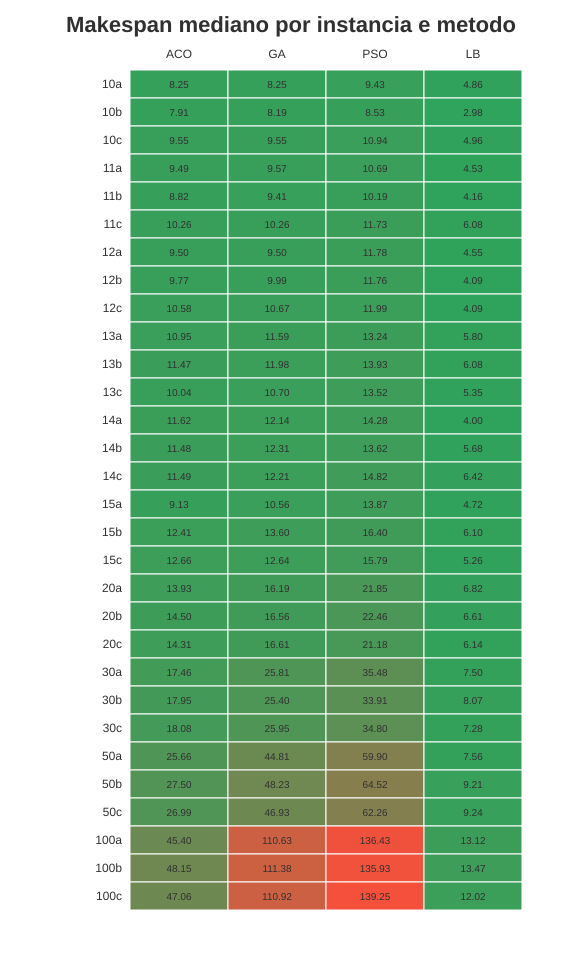
\includegraphics[width=0.86\textwidth]{figs/heatmap-makespan-median.png}
  \caption{Makespan mediano por instância e método nas 30 instâncias avaliadas. Fonte: dados de `src/data/results/'.}
  \label{fig:heatmap-makespan}
\end{figure}

Esse resultado favorece a interpretação de que a construção probabilística com feromônio tridimensional aproveitou melhor a estrutura de dependência de sequência do problema. A interpretação deve ser delimitada: ela vale para a implementação, os parâmetros e as instâncias avaliadas. Não demonstra que ACO domina GA ou PSO em todas as variantes de TSP ou em todos os cenários de patrulha.

\subsection{Lower Bound AP}

O lower bound AP foi válido nas \TotalInstanciasComOtimo{} instâncias com ótimo conhecido: em todos os casos, o valor do bound foi menor ou igual ao ótimo por busca exaustiva. Entretanto, o bound foi frouxo. O gap médio entre o lower bound e o ótimo foi \GapLBMedio{}, com mínimo de \GapLBMinimo{} e máximo de \GapLBMaximo{}.

\begin{table}[htbp]
  \centering
  \caption{Resumo do gap entre lower bound AP e ótimo por busca exaustiva.}
  \label{tab:lb-gap}
  % Generated by scripts/gerar-metricas-monografia.py; do not edit manually.
% Source: src/data/results via scripts/gerar-metricas-monografia.py.
\begin{tabular}{lr}
\toprule
Metrica & Valor \\
\midrule
Gap medio LB$\to$BF & 51{,}36\% \\
Gap minimo & 40{,}79\% \\
Gap maximo & 65{,}35\% \\
Instancias avaliadas & 18 \\
Violacoes LB $\leq$ BF & 0 \\
\bottomrule
\end{tabular}

\end{table}

A frouxidão é esperada: a redução $c'_{j,k}=\min_i G[i][j][k]$ remove parte do contexto angular, escolhendo para cada transição o melhor nó anterior possível. Isso torna o bound barato e válido, mas pouco informativo como aproximação do ótimo do TSP-SD-ATP.

\subsection{Tempo Computacional}

O ganho de qualidade do ACO vem acompanhado de maior custo computacional. Nas instâncias de 100 pontos, o tempo médio de otimização do ACO ficou em torno de \TempoOtimizacaoACOCemMedioSegundos{}, enquanto a maior média por instância do GA foi \TempoOtimizacaoGAMaxCemMs{} e a do PSO foi \TempoOtimizacaoPSOMaxCemMs{}. A Tabela~\ref{tab:tempo-100} mostra as razões por instância.

\begin{table}[htbp]
  \centering
  \caption{Tempo médio de otimização em instâncias de 100 pontos.}
  \label{tab:tempo-100}
  \scriptsize
  % Generated by scripts/gerar-metricas-monografia.py; do not edit manually.
% Source: src/data/results via scripts/gerar-metricas-monografia.py.
\begin{tabular}{lrrrrr}
\toprule
Instancia & ACO ms & GA ms & PSO ms & ACO/GA & ACO/PSO \\
\midrule
100a & 4262{,}06 & 38{,}82 & 76{,}24 & 109{,}78x & 55{,}91x \\
100b & 4276{,}55 & 36{,}27 & 75{,}25 & 117{,}89x & 56{,}83x \\
100c & 4266{,}55 & 39{,}37 & 73{,}84 & 108{,}36x & 57{,}78x \\
\bottomrule
\end{tabular}

\end{table}

\begin{figure}[htbp]
  \centering
  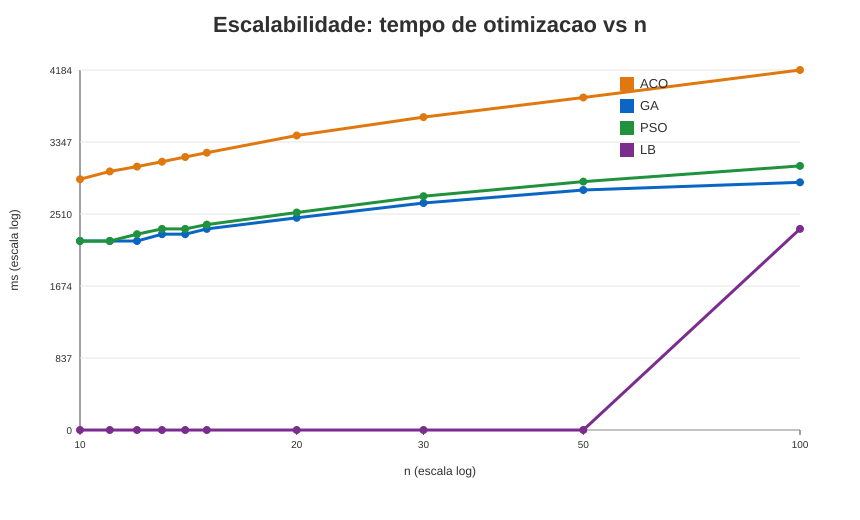
\includegraphics[width=0.92\textwidth]{figs/scalability-runtime.png}
  \caption{Escalabilidade temporal dos métodos por tamanho de instância. Fonte: dados de `src/data/results/timing/'.}
  \label{fig:runtime}
\end{figure}

\begin{figure}[htbp]
  \centering
  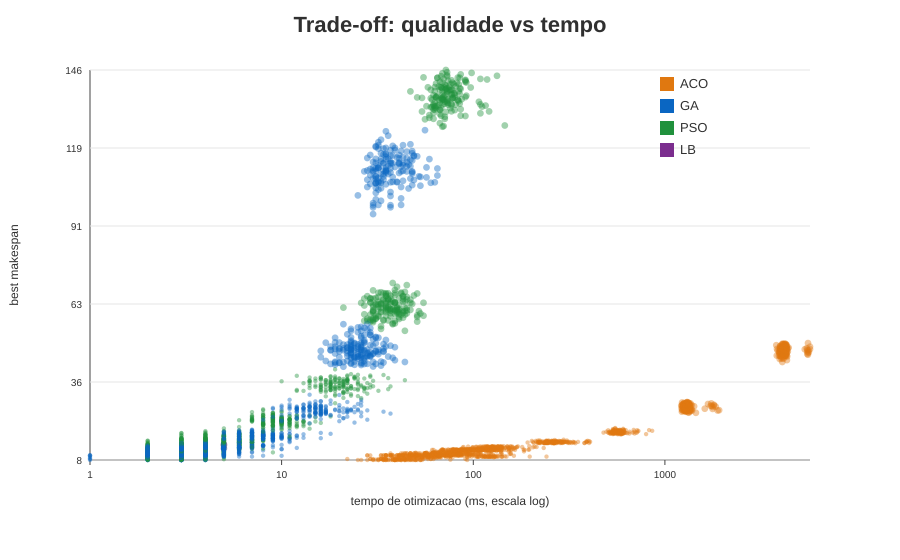
\includegraphics[width=0.92\textwidth]{figs/scatter-quality-vs-time.png}
  \caption{Trade-off entre qualidade de solução e tempo de otimização. Fonte: dados de `src/data/results/'.}
  \label{fig:tradeoff}
\end{figure}

Para patrulhamento com drones, esse trade-off é central. Se a rota puder ser planejada offline, o ACO pode ser preferível pela qualidade. Se a rota precisar ser recalculada rapidamente, o GA oferece uma alternativa muito mais barata, embora com makespan médio maior nas instâncias avaliadas.

\subsection{Estabilidade e Convergência}

A variabilidade entre sementes também difere entre os métodos. O ACO apresentou boa qualidade média e estabilidade nas instâncias grandes, mas com custo temporal elevado. O GA foi rápido, porém produziu soluções de maior makespan médio. O PSO teve o pior desempenho de qualidade neste desenho experimental, resultado compatível com a limitação da codificação por \textit{random keys}: a ordenação de valores contínuos nem sempre preserva adjacências úteis para uma rota com custos de tripletas.

\begin{figure}[htbp]
  \centering
  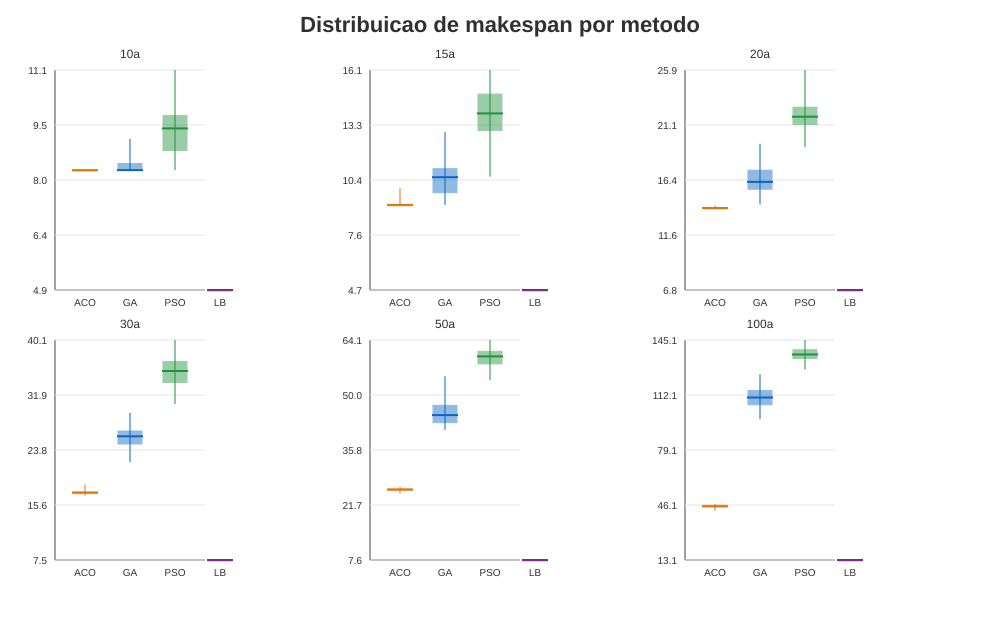
\includegraphics[width=0.92\textwidth]{figs/boxplot-estabilidade.png}
  \caption{Distribuição do makespan por método e tamanho, considerando as sementes estocásticas. Fonte: dados de `src/data/results/'.}
  \label{fig:estabilidade}
\end{figure}

\begin{figure}[htbp]
  \centering
  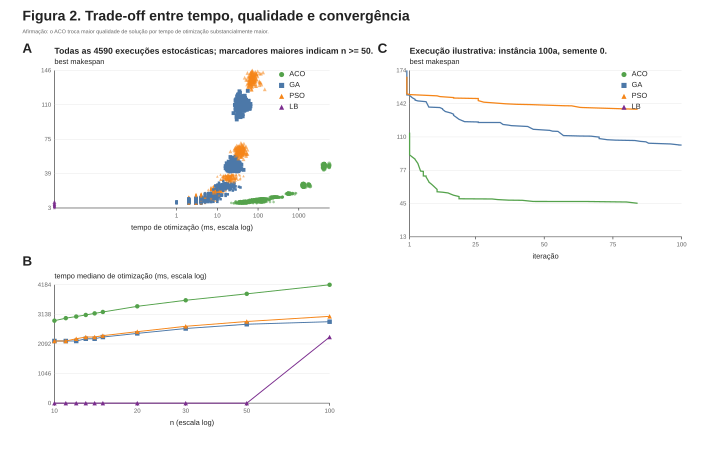
\includegraphics[width=0.92\textwidth]{figs/fig-runtime-convergence.png}
  \caption{Comportamento agregado de convergência dos métodos ao longo das execuções. Fonte: dados de evolução em `src/data/results/evolution/'.}
  \label{fig:convergencia}
\end{figure}

\subsection{Análise Estatística}

A comparação estatística seguiu Demšar \cite{demsar2006statistical}. Para cada uma das \TotalInstancias{} instâncias, foi calculada a mediana do makespan por método; em seguida, os métodos foram ranqueados por instância. O teste de Friedman com correção de Iman--Davenport rejeitou a hipótese nula de equivalência entre os métodos: $F(\FriedmanDFOne{},\FriedmanDFTwo{})=\FriedmanStatistic{}$, com $p=\PValorImanDavenport{}$.

Os ranks médios foram ACO=\RankMedioACO{}, GA=\RankMedioGA{} e PSO=\RankMedioPSO{}. O pós-teste de Nemenyi, com diferença crítica $CD=\CDNemenyi{}$ para $\alpha=0{,}05$, indicou diferença significativa nos três pares: ACO--GA, ACO--PSO e GA--PSO. O teste de Wilcoxon pareado com correção de Bonferroni--Holm também rejeitou a hipótese nula nos três pares.

\begin{figure}[htbp]
  \centering
  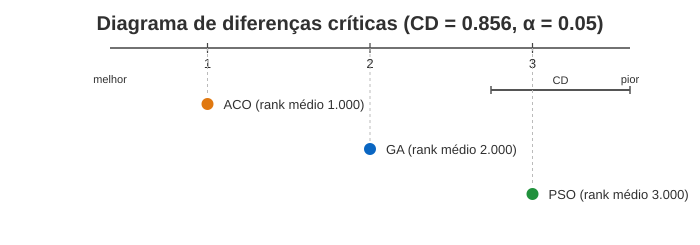
\includegraphics[width=0.80\textwidth]{figs/cd-diagram.png}
  \caption{Diagrama de diferença crítica para os ranks médios de makespan. Fonte: `scripts/analise-estatistica.py'.}
  \label{fig:cd-diagram}
\end{figure}

\subsection{Limitações Metodológicas}

Os resultados devem ser interpretados dentro do desenho experimental. Primeiro, as instâncias são sintéticas e geradas em um plano normalizado; elas não capturam obstáculos, vento, autonomia de bateria, zonas proibidas ou prioridades reais de patrulha. Segundo, os hiperparâmetros foram fixados para todos os métodos. ACO, GA e PSO poderiam ter desempenho diferente sob ajuste sistemático por instância. Terceiro, os métodos não usam a mesma codificação: GA usa permutação direta, PSO usa \textit{random keys}, e ACO constrói rotas por transições probabilísticas tridimensionais. Essa diferença é parte do desenho comparativo, mas limita inferências causais sobre a superioridade intrínseca de uma meta-heurística.

Por fim, a busca exaustiva cobre apenas as instâncias `10a' a `15c'. Para instâncias maiores, não há ótimo conhecido. O lower bound AP ajuda a oferecer uma referência, mas sua frouxidão impede tratá-lo como aproximação apertada do ótimo. As conclusões, portanto, descrevem o desempenho observado nas implementações e instâncias avaliadas, não uma ordenação universal entre GA, PSO e ACO.
